

\subsection{Основные типы соединений галогенов в высших степенях окисления, способы получения, химическое поведение, электронное и геометрическое строение молекул.}

\subsubsection*{Межгалогенные соединения}

\textbf{Способы получения}

1)Прямой синтез

$$Cl_2 + 5F_2 \rightarrow 2CiF_5 (350^{\circ}, 250 atm)$$
$$Br_2 + 5F_2 \rightarrow 2BrF_5 (>150^{\circ})$$
$$I_2 + 5F_2 \rightarrow 2IF_5 (20^{\circ})$$
$$I_2 + 7F_2 \rightarrow 2IF_7 (250-300^{\circ})$$

2) Из сложных веществ

$$MCl_{tv} + 4F_2 \rightarrow MF_{tv} + ClF_5(100-300^{\circ})$$
$$KBr + F_2 \rightarrow KF_{tv} + BrF_5$$
$$I_2 \rightarrow IF_5 (kat=AgF,ClF_3, BrF_3)$$
$$KI + 4F_2 \rightarrow KF_{tv} + 2IF_7$$
$$PdI_2 + 8F_2 \rightarrow PdF_2 + 2IF_7$$
В частности фторирование низшего фторида:
$$ClF_3 + F_2 \rightarrow ClF_5$$

\textbf{Химические свойства}

$ClF_5, BrF_5, IF_7$ - исключительно сильные фторирующие агенты, $IF_5$ - более мягкий

$$ClF_5 + 2H_2O \rightarrow ClO_2F + 4HF$$
$$ClF_5 + MeF_5 \rightarrow [ClF_4]^+[MeF_6]^-(Me= Al,Sb)$$

$$BrF_5 + 3H_2O \rightarrow HBrO_3 + 5HF (CH_3CN)$$
$$BrF_5 + CsF \rightarrow CsBrF_6\downarrow$$
$$BrF_5 + 2SbF_5 \rightarrow[BrF_4]^+[Sb2F11]^-$$
$$BrF_5 + SO_3 \rightarrow [BrF_4]^+[SO_3F]^-$$

$IF_7$ - с большинством простых веществ;

$$IF_7 + H_2O \rightarrow IOF_5 + 2HF$$
$$2IF_7 + SiO_2 \rightarrow 2IOF_5 + SiF_4 (100^{\circ})$$
$IF_5$ - донор фторид-иона($AsF_5,SbF_5$), акцептор фторид-иона ($CsF, NOF$)

$$IF_5 \rightarrow [IF_4]^+(c\ SbF_5)$$
$$IF_5 \rightarrow [IF_6]^-(c\ NOF)$$

Часто фторирование до частично фторированных аддуктов:

$$IF_5 + KMnO_4 \rightarrow MnO_3F + IOF_3 + KF$$

Образует аддукты с $XeF_2,\ XeF_4$

$$IF_5 + 3H_2O \rightarrow HIO_3 + 5HF$$
$$IF_5 + 6KOH_{aq}\rightarrow KF_{aq}+ KIO_{3(aq)} + H2O$$

С простыми веществами:

B, P, As, Sb - воспламеняются;//
Mo, W - загораются при нагревании или бурно реагируют.

\textbf{Электронное и геометрическое строение}

Определяется методом Гиллеспи:\\

$XF_5 - AB_5E$ - квадратная пирамида, где центральный атом расположен чуть ниже плоскости 4-ч атомов F в основании пирамиды. ($C_{uv}$)

$IF_7$ пентагональная бипирамида ($D_{5h}$)

$AB_7$ с небольшими искажениями.

\subsubsection*{Оксиды}
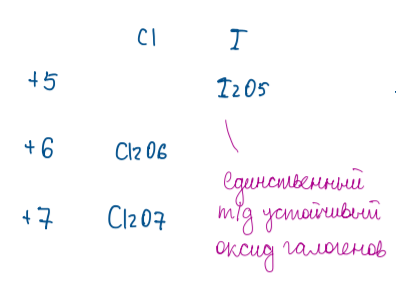
\includegraphics{images/5v1.png}

Br - очень неустойчивый в высших степенях окисления, немного информации о $Br_2O_5$:

Бесцветное твердое вещество, стабильно при температуре ниже $-20^{\circ}$;\\
Cтруктура $O_2Br-O-BrO_2$,  каждая $BrO_3$-группа пирамидальная с атомом $Br$  вершине.\\
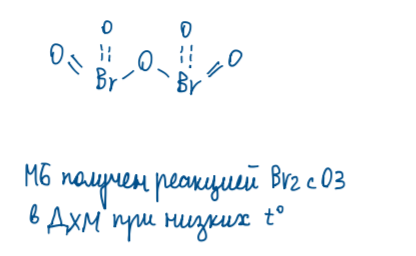
\includegraphics{images/5v2.png}

\textbf{Получение}

$$2ClO-2 + 2O_3 \rightarrow Cl_2O_6 + 2O_2$$
$$HClO_4 + H_3PO_4 \rightarrow Cl_2O_7 + HPO_3/(-10^{\circ})$$
$$HIO_3 \rightarrow I_2O_5 + H_2O$$
($I_2O_5$ можно получить разложением неустойчивых $I_4O_9,I_2O_4$ или $I_2 + O_2$(тлеющий разряд))

\textbf{Химические свойства}

$$Cl_2O_6 + H_2O \rightarrow HClO_3 + HClO_4$$
$$Cl_2O_6 + HF_{bezvodn}\leftrightarrow FClO_2 + HClO_4$$
$$Cl_2O_6 + Cr_2O_3/NO_xCl/NO_x \rightarrow [ClO_4]^-(x=1,2)$$
$$ Cl_2O_6 \rightarrow ClO_2 + O_2(0-10^{\circ})$$

$$Cl_2O_7 \rightarrow Cl_2 + O_2(60-70^{\circ})$$
$$Cl_2O7 +H_2O \rightarrow HClO_4$$
$$Cl_2O_7 + NaOH \rightarrow NaClO_4 + H_2O$$

$$I_2O_5 \rightarrow I_2 + O_2 (350^{\circ})$$
$$I_2O_5 + 5CO \rightarrow I_2 + 5CO_2$$
$$I_2O5 + H_2O \rightarrow HIO_3$$

\textbf{Электронное и геометрическое строение}

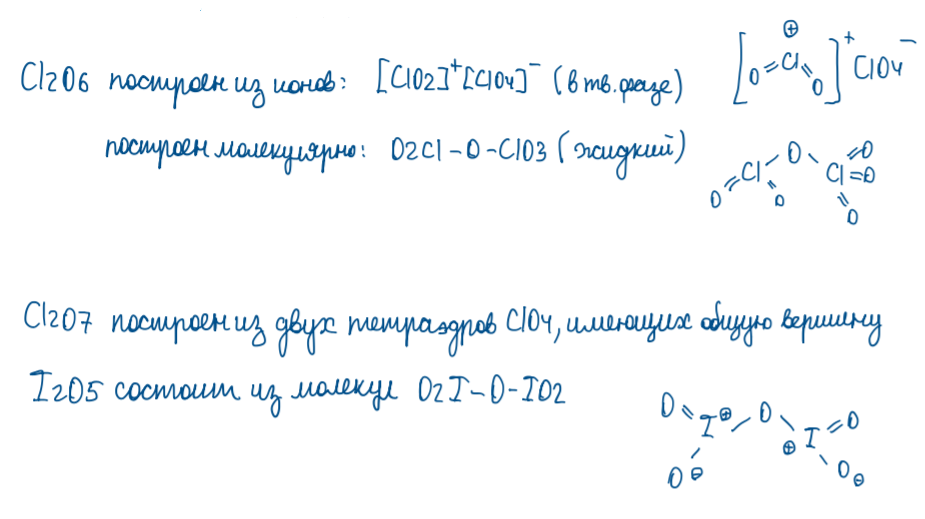
\includegraphics[scale=0.9]{images/5v3.png}

\subsubsection*{Оксокислоты и их соли}

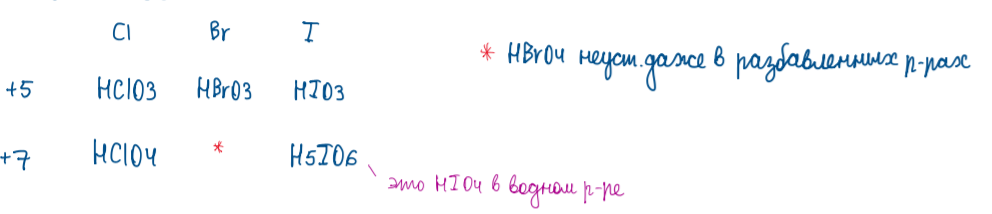
\includegraphics{images/5v4.png}

\textbf{Получение}

$$Ba(ClO_3)_2 + H_2SO_{4(razb)} \rightarrow HClO_3 + BaSO_4\downarrow$$
$$ I_2  + H_2O_2 \rightarrow HIO_3 + H_2O$$
$$I_2 + HNO3 \rightarrow HIO_3 + NO_2 + H_2O$$
$$I_2O_5 + H_2O \rightarrow HIO_3$$
$$HCl_{konc} + NaClO_{4(bezvodn)} \rightarrow HClO_4 + NaCl$$
$$Ba_3(H_2IO_6)_2 + HNO_3 \rightarrow H_5IO_6 + Ba(NO_3)_2$$
$$3KClO \rightarrow KClO_3 + 2KCl$$
$$KOH + X_2 \rightarrow KXO_3 + KX + H_2O$$
$$KXO_3 + I_2 \rightarrow KIO_3 + X_2$$
$$KClO_3\rightarrow 3KClO_4 + KCl (500^{\circ})$$
$$NaBrO_3 + F_2 + NaOH \rightarrow NaBrO_4 + NaF + H_2O$$
$$KOH + H_2O +KIO_3 + KClO \rightarrow K_2H_3IO_6 + KCl$$
$$K_2H_3IO_6 + HNO_3 \rightarrow KIO_4 + KNO_3 + H_2O$$

В степени окисления +5 окислительная способность меняется по ряду $Cl\approx Br > I$, сила кислот падает $Cl>Br>I$.

С увеличением степени окисления увеличивается сила кислот, но уменьшается окислительная активность.

В ряду $ClO_4^-\leq BrO_4^- \leq H_2IO_6^{3-}$ растут скорости реакции окисления

\textbf{Химические свойства}

Уменьшение силы кислот:
$$HClO_4 \rightarrow HBrO_3 \rightarrow HIO_3$$

Разложение:

$$HClO_3 \rightarrow HClO_4 + Cl_2 + O_2 + H_2O$$
$$HBrO_3 \rightarrow Br_2 + O_2 + H_2O$$
$$HIO_3 \rightarrow I_2O_5 + H_2O$$

ОВР: 

$$HIO_3 + H_2O_2 \rightarrow I_2 + O_2 + H_2O$$

Степень окисления +7 - сильные окислители ($HClO_4$ только в концентрированных растворах)

$$H_5IO_6 + HCl \rightarrow HIO_3 + Cl_2 + H_2O$$
$$H_5IO_6 + K_2CO_3 \rightarrow K_2H_3IO_6 + CO_2 + H_2O$$
$$K_2H_3IO_6 + KOH \rightarrow K_3H_2IO_6 + H_2O$$

В растворе нет 5-замещенных солей

Твердые галогенаты - сильные окислители

$$S + KBrO_3 \rightarrow K_2SO_4 + Br_2 + SO_2$$
$$KXO_3 + I_2 \rightarrow KIO_3 + X_2$$
 
$KClO_3$ - бертолетова соль

$$KClO_3 \rightarrow KCl + KClO_4$$
$$KClO_3 \rightarrow KCl + O_2 (t^{\circ}, MnO_2)$$

Степень окисления +7 -- сильные окислители (но слабее, чем сами кислоты)

$$KClO_4 \rightarrow KCl + O_2 (>550^{\circ})$$

\textbf{Электронное и геометрическое строение}

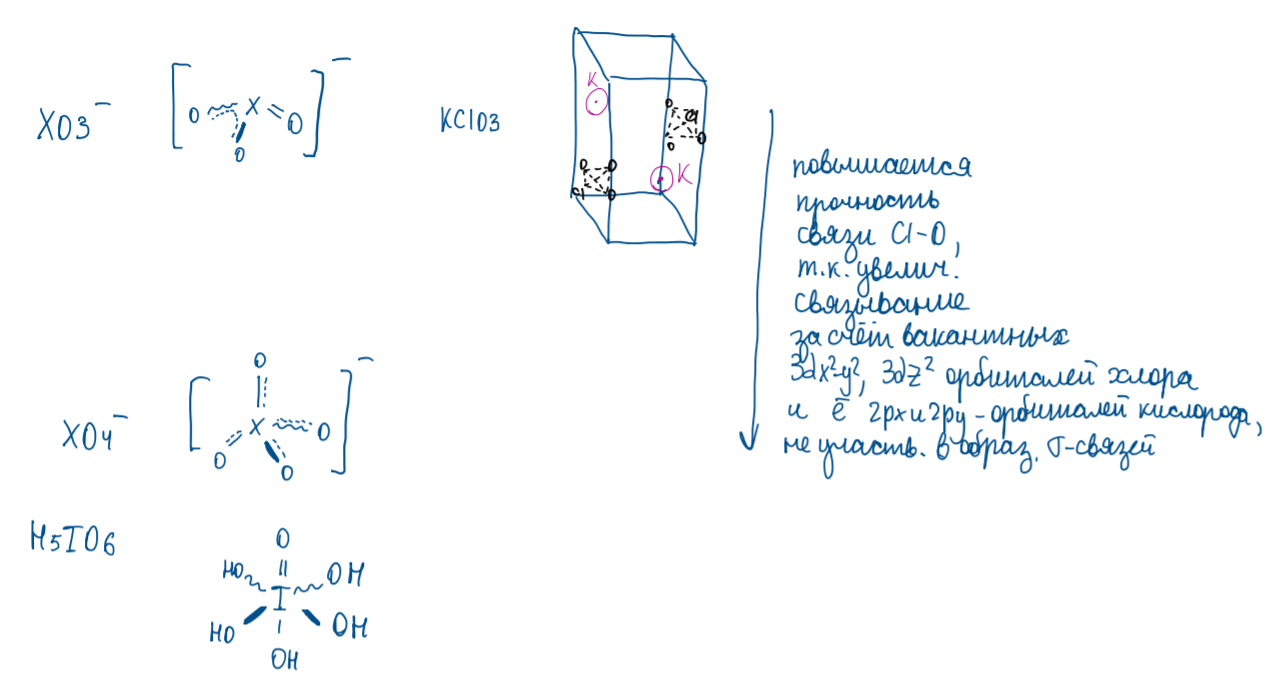
\includegraphics[scale=0.7]{images/5v5.png}
